\chapter{Introduction}
\label{chap:intro}
\textbf{In this section I will explain and summarize what my internship and intership reports were all about and give a brief outline for the following chapters.}
\section{Motivation} % why is this a non trivial problem
	
	As part of my Computer Science Curriculum in the National Engineering School of Tunis, I wanted to complete my internship in a company that is in line with my professional orientation. I did not choose a Telecommunications Company because I wanted to switch to the field of Telecommunications afterwards, but because the mission that was proposed to me was consistent with my professional goals. \\  

	Indeed, my primary mission was to observe the environment and interaction of Tunisie Telecom's employees and their discipline and hard work, I also discovered several new tools and techniques that were above me, I also learned of several devices and techniques employed by Tunisie Telecom to guarantee their Networks are top notch, it was a great opportunity for me to actually be in such an environment, which gave me more courage as a student to see myself becoming a software engineer. \\
	
	In a second time, I had to design a Web Platform, which is accessible locally. Its role is to enable all Tunisie Telecom staff of Creating, Storing, Updating and Deleting different entries of a Fiber Optics stock management program according to their User Type, putting as a priority the simplicity and efficiency of the Web Platform.\\

	Finally,  I'm very satisfied of this internship because it introduced me to a lot of new concepts like HTML, CSS, BootStrap, PHP, MySQL, LAMP stack, Linux and even Git Version Control Systems in a domain that I love. And also allowed me to highlight my skills aquired during my Software Engineering year of studies. \\ 

The place where I did the Internship is shown in Figure~\ref{fig:test1}.
\begin{figure}[ht!] % supposedly places it here ...
  \centering
  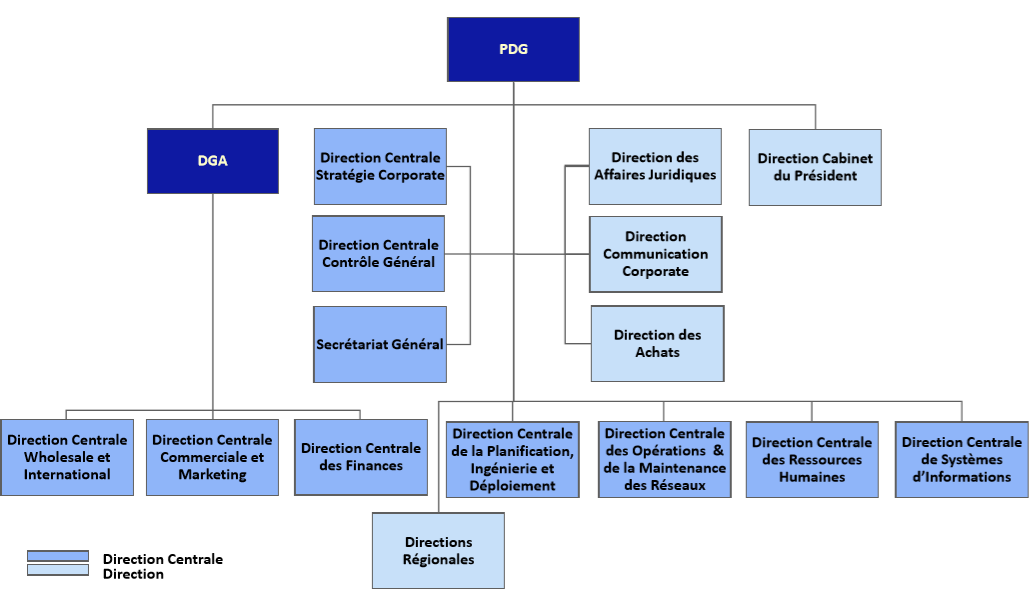
\includegraphics[width=0.6\linewidth]{test_image_goku}
  \caption[Where I Did the Internship]{Tunisie Telecom \index{Goku il-king}}%
  \label{fig:test1}
\end{figure}

	This is an Image from Google Maps of the Digital Transmission Center (Centre de Transmission Numérique - CTN) of Tunisie Telecom based in Place Pasteur, Belvedere, hereafter noted DTC. Where I did my Internship.

% \textbf{Note that you may have multiple \texttt{{\textbackslash}include} statements here, e.g.\ one for each subsection.}\cofeBm{0.7}{1}{0}{3cm}{-1cm}

\section{Aims and Objectives - Outline} 

	Besides this Chapter~\autoref{chap:intro} and the Conclusion~\autoref{chap:conc}. There are two main chapters:
	\begin{itemize}
	\item In Chapter~\autoref{chap:org},I will Introduce Tunisie Telecom DTC Belvedere, the company's history and its field of Telecommunications and the things I saw there, as well as the Data Unit (Unité Data) branch, that is responsible for dealing with big companies and clients in which I worked.
	\item In Chapter~\autoref{chap:app}, I will Introduce the Problem that we faced in Tunisie Telecom alongside the Solution I came up with, It's analysis, conception and realisation alongside the tools I learned throughout the way.
	%What's my aims and objectives??

	\end{itemize}
% \blindtext

% \begin{table*}\centering
% \ra{1.3}
% \begin{tabular}{@{}rrrrcrrr@{}}\toprule
% & \multicolumn{3}{c}{$w = 8$} & \phantom{abc}& \multicolumn{3}{c}{$w = 16$} \\
% \cmidrule{2-4} \cmidrule{6-8} 
% & $t=0$ & $t=1$ & $t=2$ && $t=0$ & $t=1$ & $t=2$\\ \midrule
% $dir=1$\\
% $c$ & 0.0790 & 0.1692 & 0.2945 && 0.3670 & 0.7187 & 3.1815\\
% $c$ & -0.8651& 50.0476& 5.9384&& -9.0714& 297.0923& 46.2143\\
% $c$ & 124.2756& -50.9612& -14.2721&& 128.2265& -630.5455& -381.0930\\
% $dir=0$\\
% $c$ & 0.0357& 1.2473& 0.2119&& 0.3593& -0.2755& 2.1764\\
% $c$ & -17.9048& -37.1111& 8.8591&& -30.7381& -9.5952& -3.0000\\
% $c$ & 105.5518& 232.1160& -94.7351&& 100.2497& 141.2778& -259.7326\\
% \bottomrule
% \end{tabular}
% \caption{A Beautiful and Complex Table}\label{tab:sometable}
% \end{table*}

% A beautiful table is shown in Table~\ref{tab:sometable}, data from \citet{Ebejer2012} (when citing as part of text, otherwise \citep{Ebejer2012}).


% \blindtext

% % \begin{figure}[ht!] % supposedly places it here ...
% %   \centering
% %   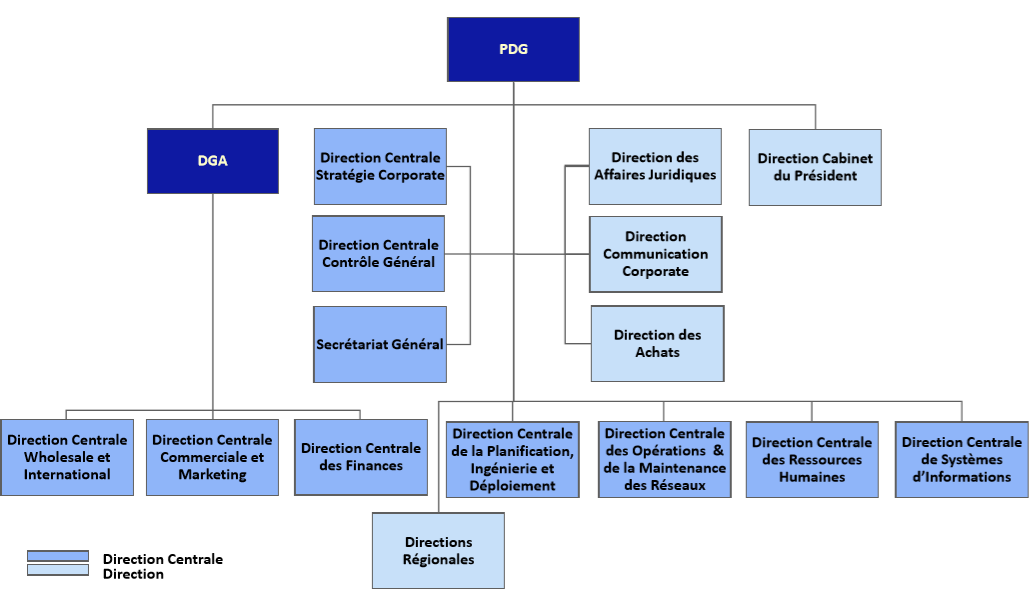
\includegraphics[width=0.6\linewidth]{test_image_goku}
% %   \caption[This is the short caption for List of Figures]{A test figure.  This caption is huge, but in the list of figures only the smaller version in the square brackets will appear.\index{Goku il-king}}
% %   \label{fig:test1}
% % \end{figure}



% \section{Proposed Solution} 

% \blindtext
% \blindtext

% \begin{figure}[!ht]
%     \centering
%     \subbottom[Goku]{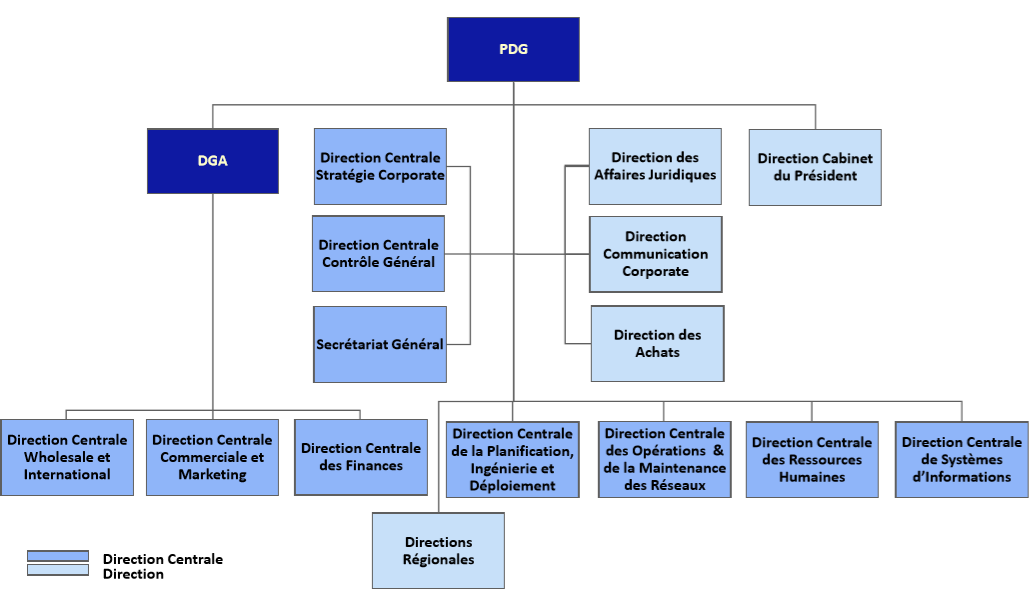
\includegraphics[width=0.3\textwidth]{test_image_goku}}\qquad
%     \subbottom[More Goku]{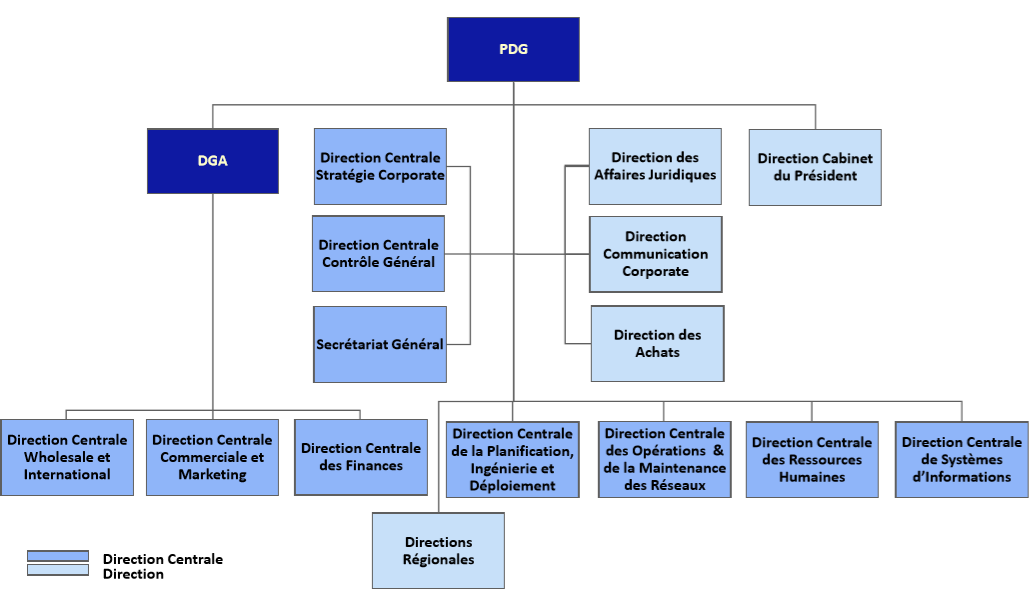
\includegraphics[width=0.3\textwidth]{test_image_goku}}%
%     \caption[Short Caption]{The same super saiyan. Two times.}        
%     \label{fig:test2}
% \end{figure}

% Two figures shown side by side are shown in Figure~\ref{fig:test2}.

% \subsection{Showing the Use of Acronyms}

% In the early nineties, \acs{GSM} was deployed in many European countries. \ac{GSM} offered for the first time international roaming for mobile subscribers. The \acs{GSM}’s use of \ac{TDMA} as its communication standard was debated at length. And every now and then there are big discussion whether \ac{CDMA} should have been chosen over \ac{TDMA}.

% If you want to know more about \acf{GSM}, \acf{TDMA}, \acf{CDMA} and other acronyms, just read a book about mobile communication. Just to mention it: There is another \ac{UA}, for testing.


% \section{Document Structure}

% \blindtext
